\chapter{Related work}


\todo[inline]{mention here rhyme generating tools like rhymezone}
\todo[inline]{Is it OK that this chapter uses IPA but IPA is explained in the next sections?}
\todo[inline]{uviest do related works aj 4 metody detekcie rymov od plechaca? ale vsetky priklady su machine learning okrem sparsaru}
\subsection{Rhyme types and literary devices}
Although everyone instinctively knows what a rhyme is and can recognize one in a poem or a song, it does not have a very precise definition. It is described as "a word that has the same last sound as another word" by Cambridge Dictionary (\cite{walter2008cambridge}) or a "literary device, featured particularly in poetry, in which identical or similar concluding syllables in different words are repeated" by \cite{literarydevices2020}. These definitions are not detailed enough to base a good algorithm off of, so let's look deeper into different rhyme types.

\paragraph{Perfect rhyme} (also true rhyme, or sometimes just "rhyme") is the most common and valued \todo{cite?} type of rhyme. It requires two conditions to be met:

\begin{itemize}
	\item last stressed vowel and all following sounds are identical
	\item immediately preceding sounds differ
\end{itemize}

It is also the only rhyme for which the definitions are consistent (for example, see \cite{bain1867manual}, \cite{vanphonological}, \cite{bergman2017litcharts}, \footnote{\url{https://en.wikipedia.org/wiki/Rhyme}}). It can be further distinguished depending on how many syllables are involved:

\begin{itemize}
	\item \textbf{Masculine} (also single, monosyllabic) -- "the commonest kind of rhyme, between single stressed syllables at the ends of verse" (\cite{oxforddict2008literary}). 
	Examples: 
	
	fly (\textipa{\underline{flaI}}) / sky (\textipa{\underline{skaI}})
	
	before (\textipa{bi-\underline{fOr}}) / explore (\textipa{Iks-\underline{plOr}})
	\footnote{For the examples, we are using IPA transcriptions because it is more comfortable for human reader.}
	\footnote{Stressed syllables are underlined. Syllables are separated with a hyphen.}
	
	\item \textbf{Feminine} (also double) -- "a rhyme on two syllables, the first stressed and the second unstressed" (\cite{oxforddict2008literary}). Examples: 
	
	bitten (\textipa{\underline{bI}-t@n}) / written (\textipa{\underline{rI}-t@n})
	
	lazy (\textipa{\underline{leI}-zi}) / crazy (\textipa{\underline{kreI}-zi})
	
	\item \textbf{Dactylic} (also triple) -- "a rhyme on three syllables, the first stressed and the others unstressed"(\cite{oxforddict2008literary}). Examples: 
	
	amorous (\textipa{\underline{æ}-m@r-@s}) / glamorous (\textipa{\underline{glæ}-m@r-@s})
	
	vanity (\textipa{\underline{væ}-nI-ti}) / humanity (\textipa{ju-\underline{mæ}-nI-ti}))
	
\end{itemize}

\paragraph{Imperfect rhyme} (also slant or half rhyme)  rhymes "the stressed syllable of one word with the unstressed syllable of another word" (\cite{bergman2017litcharts}). Examples: 

cabbage (\textipa{\underline{kæ}-bIdZ}) / ridge (\textipa{\underline{rIdZ}})

painting (\textipa{\underline{peI}-nIN}) / ring (\textipa{\underline{rIN}})

\noindent In other sources, definitions differ -- for example \cite{literarydevices2020} calls this effect "feminine rhyme".  On the other hand, \cite{oxforddict2008literary} and \cite{britannica} use the term "imperfect rhyme" for end-line consonance (see definition below) and \cite{vanphonological} uses it for end-line assonance (see definition below). For the purpose of this thesis we will work with the first definition mentioned.

\paragraph{Unaccented rhyme} (also weakened rhyme) "occurs when the relevant syllable of the rhyming word is unstressed" (\cite{britannica}). Examples: 

hammer (\textipa{\underline{hæ}-m@r}) / carpenter (\textipa{\underline{kAr}-p@n-t@r})

\noindent The difference opposed to imperfect rhyme is that here both rhyme fellows are unstressed.


\paragraph{Identical rhyme} (also rime riche) is "a kind of rhyme in which the rhyming elements include matching consonants before the stressed vowel sounds." This includes "rhyming of two words with the same sound and sometimes the same spelling but different meanings e.g seen (\textipa{\underline{sin})}/ scene (\textipa{\underline{sin}}). The term also covers word‐endings where the consonant preceding the stressed vowel sound is the same: compare (\textipa{k@m-\underline{pEr}}) / despair (\textipa{dI-\underline{spEr}})." (\cite{oxforddict2008literary}). It is generally considered not as good as perfect rhyme because it is too predictable for the listener\footnote{\url{https://literaryterms.net/rhyme/}}.

\paragraph{Forced rhyme} (also near rhyme) "includes words with a close but imperfect match in sound in the final syllables" \cite{bergman2017litcharts}. Examples: 

green (\textipa{\underline{grin}}) / fiend (\textipa{\underline{find}})

hide (\textipa{\underline{haId}}) / mind (\textipa{\underline{maInd}})

\noindent This includes the case when spelling in changed in order to make the rhyme work, e.g. truth (\textipa{\underline{truT}}) / endu'th (\textipa{en-\underline{duT}}) (a contraction of "endureth"). It can also refer to using unnatural word order to get the rhyming word at the end of the line (\cite{bergman2017litcharts}) but we will not make use of this interpretation in this thesis.

\paragraph{Assonance} is "repetition of stressed vowel sounds within words with different end consonants" (\cite{britannica}). Examples:	

quite (\textipa{\underline{kwaIt}}) / like (\textipa{\underline{laIk}})

free (\textipa{\underline{fri}}) / breeze (\textipa{\underline{briz}})

\noindent The term itself defines a literary device applicable anywhere in the poem but when used at the end of verse, it can sometimes be considered a rhyme (under various names) by sources like \cite{vanphonological}, \cite{bergman2017litcharts} and others.

\paragraph{Consonance} is "the recurrence or repetition of identical or similar consonants" (\cite{britannica}). Examples: 

country (\textipa{\underline{k@n}-tri}) / contra (\textipa{\underline{kAn}-tr@})

hickory dickory dock (\textipa{\underline{hI}-k@-ri \underline{dI}-k@-ri \underline{dAk}})

\noindent Similarly as assonance, it applies to repetition anywhere. When seen at the end of verse, it can be considered a rhyme and again, various terms are used, perhaps the most common is "pararhyme" (\cite{britannica}, \cite{oxforddict2008literary}).
\newline

The last two terms may seem as more of a tool for poets than songwriters. Surprisingly, they have found their way into song lyrics and have become a standard in genres like hip hop according to \cite{vanphonological}. From the creative point of view, it is not less sophisticated rather it enriches rhyme as we know it (\cite{brogan2016poeticterms}).
\todo[inline]{Mention here we're not using it as a rhyme - or maybe if it will be highlighted in the visualization?}
\todo[inline]{uviest to tam jasnejsie? definicie zo slovnikov nie su dost vyhranene (ex. consonance - nehoduju sa vowels!)
}

Other rhyme types exist e.g. eye rhyme where "the spellings of the rhyming elements match, but the sounds do not, e.g. love (\textipa{\underline{l@v}}) / prove (\textipa{\underline{pruv}})" (\cite{oxforddict2008literary}). We will be omitting them because we did not consider them relevant for song lyrics or the purpose of this thesis.

\todo[inline]{spomenut ze nevieme zistit ci to spevak nevyslovi inak ,ze moze hltat bezprizvucne slabiky viac naraz
}


\section{Rhyme detection tools}
\todo[inline]{Pridat nejaky nastroj co pouziva len CMU dictionary}
\subsection{SPARSAR}


\subsection{Unsupervised approach}
\subsubsection*{EM algorithm}
\cite{reddy2011unsupervised} proposed a language-independent model for finding rhyme schemes in poetry. They created an unsupervised model based on EM algorithm that assigns the most probable rhyme scheme for each sequence of line-final words. It achieved good results when tested on annotated English and French corpus with poetry from 15\textsuperscript{th} to 20\textsuperscript{th} century. However its big pitfall lies in the fact that it is biased towards the rhyme schemes from golden data. It has a predefined set of all rhyme schemes found in tested data and those are the only ones it chooses from. For illustration, in a 14-line stanza it can choose from 90 schemes which is only 0.00005\% of all possible options. In 29\% of cases from French corpus it has only one choice.\footnote{\url{http://versologie.cz/talks/2017basel/}}

\subsubsection*{RhymeTagger}
\cite{plechavc2018collocation} came with a collocation-driven alternative named RhymeTagger. It uses the same dataset as the previous approach with addition of a larger Czech poetry corpus\footnote{\url{https://github.com/versotym/corpusCzechVerse}}. Each line-final word is transcribed into phonetic transcription and split into components -- \gls{syllable_peak} for each syllable and \gls{consonant_clusters} in between. In the "expectation" step, probabilities for each component pair are calculated based on their co-occurrence in line-final words, e.g. conditional probability of rhyme based on peak component pair \textipa{@U:@U} will be very high but for consonant component pair k:r quite low. These statistics for component pairs are then used in the "maximization" step to calculate the probability for line-final word pair as a combined probability of all their components (paired by means of usual association measure). If the probability of two words is above a given threshold they are considered a rhyme. After all such pairs are classified, probabilities are iteratively recalculated in the EM cycle. 

For words that were not successfully classified with this method, there is a fallback. The author observed that some words are now pronounced differently than they were during the Shakespearean era they were written in and therefore using current pronunciation dictionaries may ruin the original rhyme, e.g. original near (\textipa{nE:r}) / there (\textipa{DE:r}) vs. contemporary near (\textipa{nI:r}) / there (\textipa{DE:r}). Original pronunciation can be therefore inferred from words with similar orthography. He calculated rhyme probability given final character trigrams, which helped achieve higher recall. Although other methods may have better precision, collocation-driven approach wins in recall as seen in \ref{screenshotRT}. This method does not take into account meter.

For evaluation, they used precision, recall and F-score calculated as follows:

\[PRECISION=\frac{true\ positives}{true\ positives+false\ positives}\]

\[RECALL=\frac{true\ positives}{true\ positives+false\ negatives}\]

\[F-SCORE=\frac{2*PRECISION*RECALL}{PRECISION+RECALL}\]

For an intuitive view, the reader can imagine precision as how many of algorithm's rhymes were actually rhymes and recall as how many rhymes were discovered. F-score describes the trade-off between the two.

\begin{figure}[h]\centering
	\includegraphics[scale=0.4]{../img/plechac_eval.png}
	\caption[RhymeTagger evaluation]{Evaluation of RhymeTagger on English corpus in comparison with EM algorithm and simple rule-based approach. The x axis is the year when the tested poem was written, the y axis are the evaluation scores as described above. Reproduced from \cite{plechac2017presentation}.}
	\label{screenshotRT}
\end{figure}
\todo[inline]{Popisat preco nejdu ich data pouzit na testovanie mojej detekcie rymov}

\subsubsection*{Deep-speare}
As a part of their \gls{sonnet} \gls{quatrain} generating model, \cite{lau2018deep} have implemented a Rhyme component that identifies and generates rhymes. It is a unidirectional forward \gls{LSTM} (\cite{hochreiter1997long}) that learns to separate rhyming word pairs from non-rhyming. They generate input by pairing one line-final word with the other three from the same quatrain. Since the rhyme scheme of a \gls{sonnet} \gls{quatrain} is always \textit{abab} this will result in one rhyming pair and two non-rhyming. Additional non-rhyming pairs are generated with random word sampling. Then the model with margin-based loss learns the margin separating the best pair from all the others. It returns a cosine similarity score that estimates how well do two words rhyme.

To evaluate this model, authors used phoneme matching with CMUdict \footnote{\url{http://www.speech.cs.cmu.edu/cgi-bin/cmudict}} and the EM model from \cite{reddy2011unsupervised} trained on their own data and they were able to outperform both based on F1 score.



\section{Visualization tools}
In the following section, we will describe existing visualization tools for poetry. Software mentioned below focuses on poems, however song lyrics can be considered just a more structurally relaxed version of a regular poem.
\subsection{Poem Viewer}
Quite complex and comprehensive visualization tool is Poem Viewer \cite{Abdul2013}. With no need for complicated installations it is easily available for the writers as a web-based application as shown in Figure \ref{screenshotPV}. Unfortunately, at the time of writing this thesis the upload of custom text was not working. Luckily, this is still an ongoing project so this might be just a temporary issue. Nevertheless there are some default poems available to demonstrate this software's capabilities.
\begin{figure}[h]\centering
	\includegraphics[scale=0.24]{../img/ScreenshotPV.png}
	\caption{Screenshot from Poem Viewer tool -- visualizing Love by Elizabeth Barrett Browning.}\label{screenshotPV}
\end{figure}

\begin{figure}[h]\centering
	\includegraphics[scale=0.4]{../img/snapshotPV_options.pdf}
	\caption{Available options and their default mappings in Poem Viewer.}\label{screenshotPV-options}
\end{figure}

Most of the analyzed features (shown in Figure \ref{screenshotPV-options} focus on the phonetic aspects of the poem. After phonetic transcription to IPA users can analyze consonant features, vowel length and position, stress, syllables, word classes and sentiment using color codes and markers. A second layout offers six different graphs/animations of tongue positions during each verse. Arcs are used to mark end rhyme, alliteration, assonance, consonance, their particular frequencies and repeating words.


Overall this software, although very elaborate, appears crammed and confusing for an inexperienced user. Moreover, it is perhaps better suited for its original use case -- a well-structured poem -- than less regular song lyrics.

\subsection{SPARSAR}
SPARSAR (\cite{Delmonte2014}) is also a very interesting tool for poetry analysis and expressive Text-to-speech conversion. It is originally designed for a thorough examination of a very strictly structured Shakespeare's sonnets. To achieve this, it has to run analyses on many levels -- and these results can be used to analyze any poem. It looks at the poem on three levels: phonetic (pronunciation, consonant and vowel tongue position, assonances, etc.), poetic (metrical structure, rhyme schemes, acoustic length, etc.), and semantic (sentiment, methaphorically linked words, anaphora, etc.).

User can choose between a window application with graphs and diagrams or a \gls{headless_mode} with .xml output files. Its main disadvantage for our use case is that it is written in Prolog and therefore is very strict on the input format and runs only under a specific older version of Ubuntu. 

\subsection{ProseVis}
This Java desktop visualization tool by \cite{Clement2013} analyzes text through
parts-of-speech, phonemes, stress, tone, and break index. These features are extracted using OpenMary Text-to-speech system (\cite{Schroder2006}) and predictive classification. The authors believe their visualization will present the features to user in a more human readable form (\cite{prosevis2017sourceforge}).

\begin{figure}[h]\centering
	\includegraphics[scale=0.24]{../img/prosevis.png}
	\caption[Comparison of two poems in ProseVis]{Comparison of two poems in ProseVis. Reproduced from \cite{prosevis2017sourceforge}.}\label{screenshotProsevis}
\end{figure}

\subsection{Poemage and RhymeDesign}
Poemage (\cite{McCurdy2015poemage}) and RhymeDesign (\cite{McCurdy2015}) are both open-source applications with focus on analysis of sonic devices and sonic topology in poetry. Poemage\footnote{\url{http://www.sci.utah.edu/~nmccurdy/Poemage/}} focuses on complex structures of words connected through some sonic or linguistic resemblance across the space of the poem. It is available for MacOS or Windows with a web version currently under development. In MacOS application RhymeDesign -- which also provides the backend for Poemage -- users can enter their poem and query for one of the default rhyme types or choose a custom rhyme type.

\begin{figure}[h]\centering
	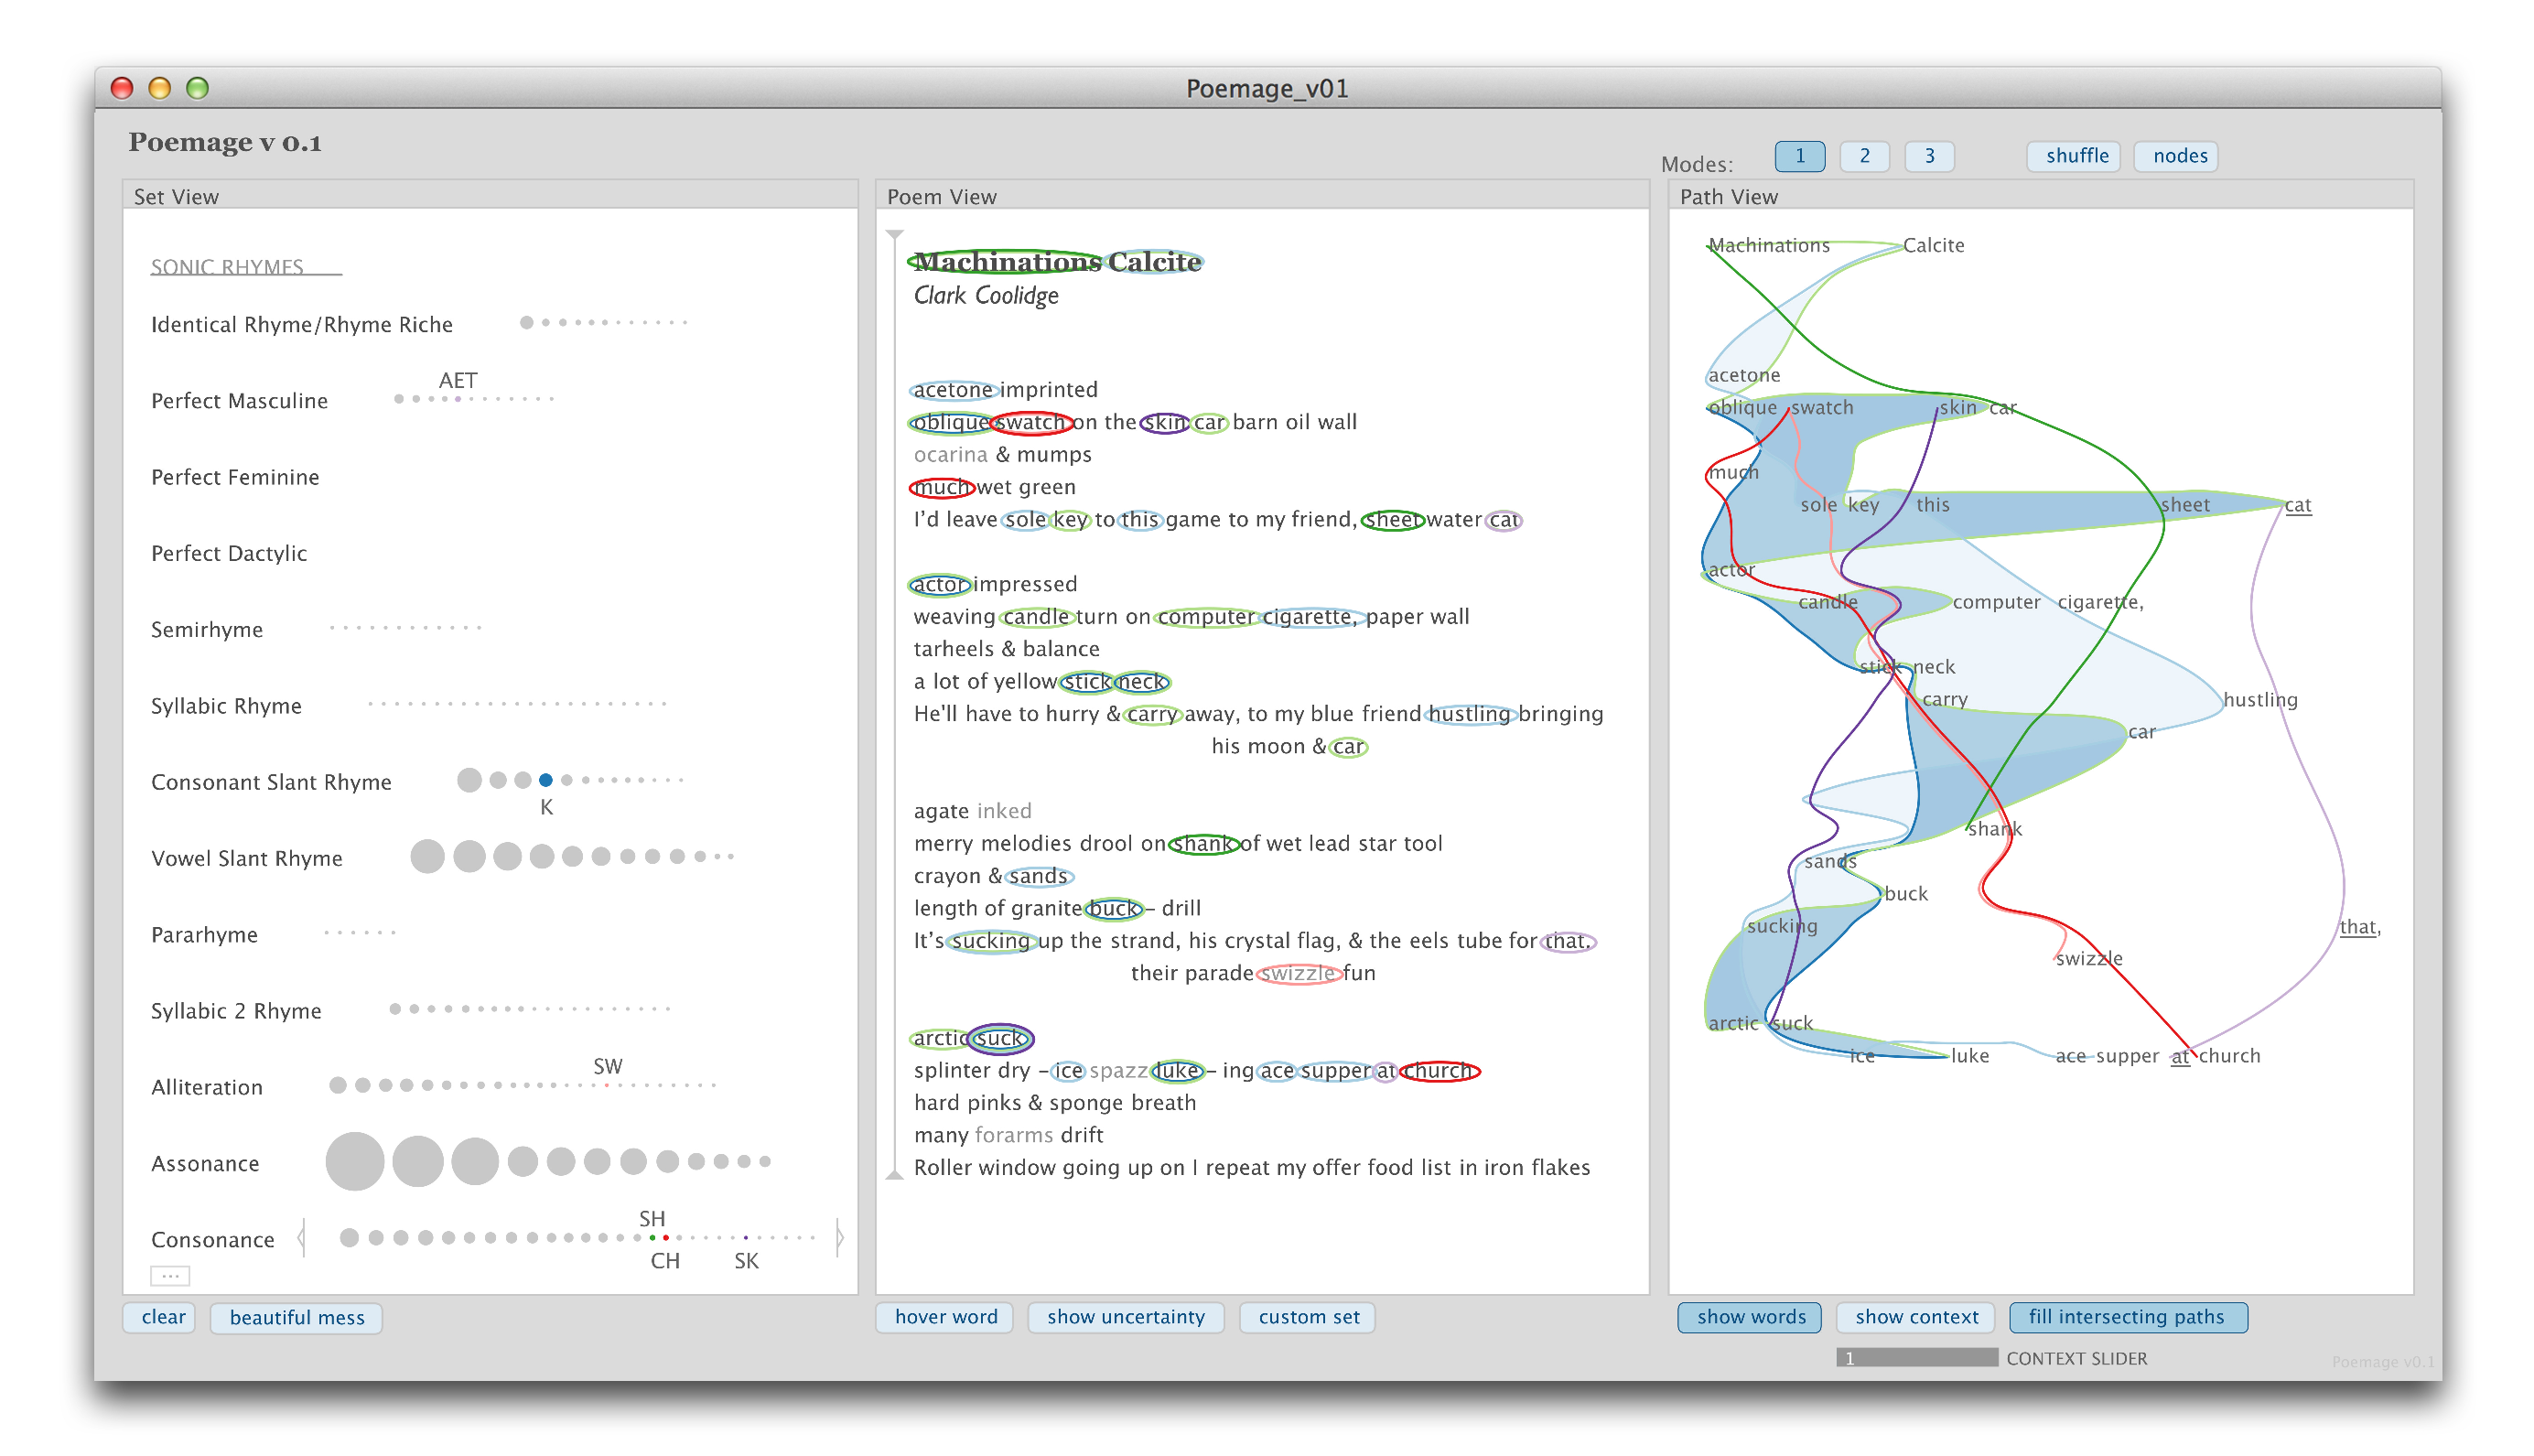
\includegraphics[scale=0.24]{../img/poemage.pdf}
	\caption{An example analysis in Poemage.}\label{screenshotPoemage}
\end{figure}

\subsection{Ambiances}
This software is unique in the fact that the analysis is integrated in the process of writing. As described in the paper \cite{Meneses2015}, writers enter the poem, receive a visualization and can control this visualization with body and hand gestures which in turn influence the poem. By such interconnection the authors aim to make Ambiances a part of the writing process and give it a chance to influence the final result. However, the actual software does not seem to be openly available.


\section{Generation tools}
\cite{lau2018deep} - learns rhyme automatically, for sonnets, results indistinguishable, apart from expert evaluation, missing emotion
\todo[inline]{generation by Reddy}